\subsection{Optical Communications System Overview}

Optical communications systems are typically composed of the components listed
in Figure \ref{fig:overview}, that is a light source, an information source, an
encoder and modulator, optics at both the transmitting and receiving side, a
transmission medium, a detector, and a receiver.

\begin{figure}[H]
	\centering
	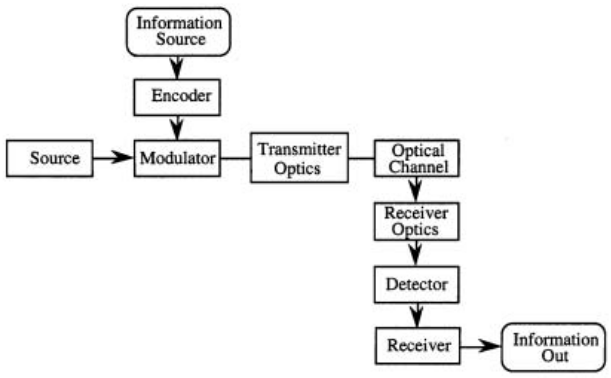
\includegraphics[width=0.8\textwidth]{images/optcommsblock}
	\caption{Generalised Block Diagram of an Optical Communications System
	\cite{mickelson_2003}}
	\label{fig:overview}
\end{figure}

\par As previously discussed, the light source used is typically an LED or a laser
diode (LD). Laser diodes offer advantages in modulation speed, power and spatial
coherence\cite{alwayn_2004}.

\par At the transmission side, the incoming source must be modulated with the data
signal. The modulation techniques used, and the most recent advances in these
techniques will be discussed within this review paper.

\par At the receiving side, a photodiode converts the incoming light signal to
an electrical signal. This is typically followed by multiple amplification stages,
and can also include circuitry for decoding the signal, or error
detection\cite{alwayn_2004}.
